\section{Software Layers}

Die folgenden Diagramme beschreiben die Umsetzung zuerst Technologie-Unabhängig und danach mit der effektiven Implementation.\\
Durchgezogene Pfeile sind dabei als synchrone Kommunikation zu verstehen. Gestrichelte Pfeile als asynchrone Kommunikation.

\subsection*{Technologie-Unabhängig}

\begin{figure}[ht!]
	\centering{
		% Graphic for TeX using PGF
% Title: /Users/michael/code/BA/dokumentation/content/sad/layers-diagram.dia
% Creator: Dia v0.97.2
% CreationDate: Tue Mar 12 22:45:08 2013
% For: michael
% \usepackage{tikz}
% The following commands are not supported in PSTricks at present
% We define them conditionally, so when they are implemented,
% this pgf file will use them.
\ifx\du\undefined
  \newlength{\du}
\fi
\setlength{\du}{15\unitlength}
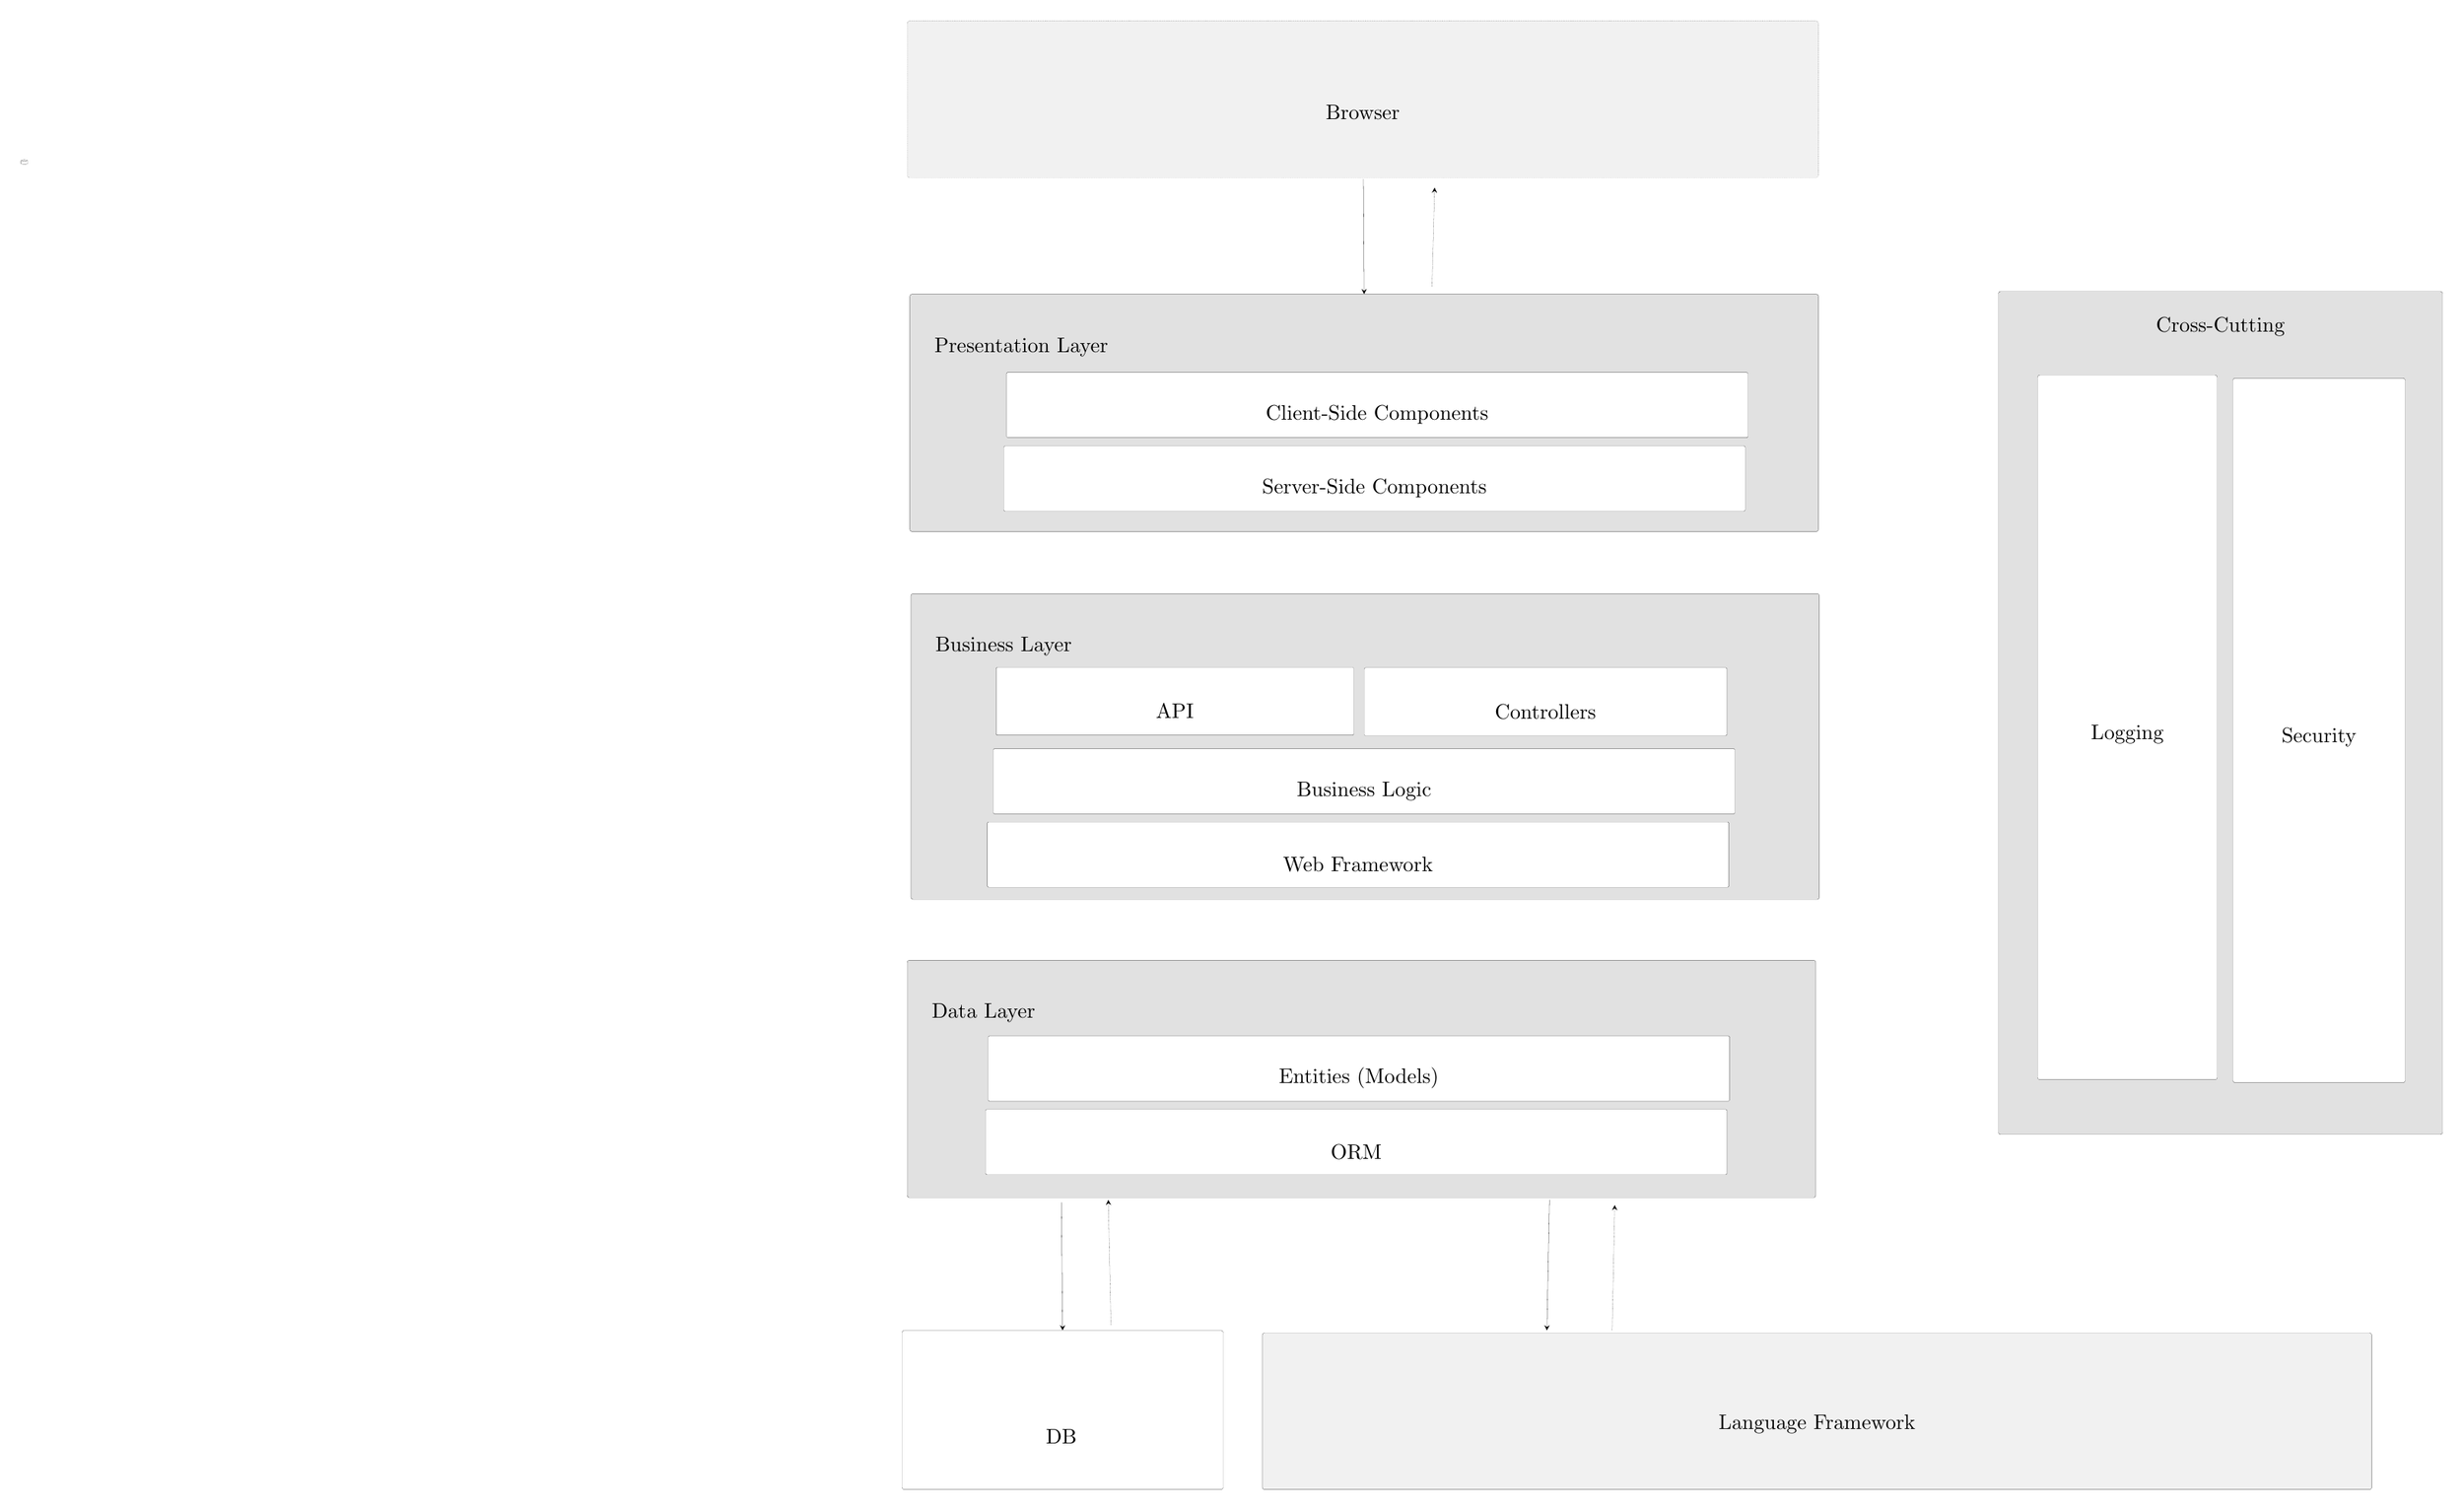
\begin{tikzpicture}
\pgftransformxscale{1.000000}
\pgftransformyscale{-1.000000}
\definecolor{dialinecolor}{rgb}{0.000000, 0.000000, 0.000000}
\pgfsetstrokecolor{dialinecolor}
\definecolor{dialinecolor}{rgb}{1.000000, 1.000000, 1.000000}
\pgfsetfillcolor{dialinecolor}
\pgfsetlinewidth{0.050000\du}
\pgfsetdash{}{0pt}
\pgfsetdash{}{0pt}
\pgfsetroundjoin
{\pgfsetcornersarced{\pgfpoint{1.000000\du}{1.000000\du}}\definecolor{dialinecolor}{rgb}{0.882353, 0.882353, 0.882353}
\pgfsetfillcolor{dialinecolor}
\fill (33.658800\du,2.925000\du)--(33.658800\du,17.034356\du)--(41.088986\du,17.034356\du)--(41.088986\du,2.925000\du)--cycle;
}{\pgfsetcornersarced{\pgfpoint{1.000000\du}{1.000000\du}}\definecolor{dialinecolor}{rgb}{0.000000, 0.000000, 0.000000}
\pgfsetstrokecolor{dialinecolor}
\draw (33.658800\du,2.925000\du)--(33.658800\du,17.034356\du)--(41.088986\du,17.034356\du)--(41.088986\du,2.925000\du)--cycle;
}% setfont left to latex
\definecolor{dialinecolor}{rgb}{0.000000, 0.000000, 0.000000}
\pgfsetstrokecolor{dialinecolor}
\node[anchor=west] at (37.373893\du,9.979678\du){};
% setfont left to latex
\definecolor{dialinecolor}{rgb}{0.000000, 0.000000, 0.000000}
\pgfsetstrokecolor{dialinecolor}
\node at (37.373893\du,3.520000\du){Cross-Cutting};
\pgfsetlinewidth{0.050000\du}
\pgfsetdash{}{0pt}
\pgfsetdash{}{0pt}
\pgfsetroundjoin
{\pgfsetcornersarced{\pgfpoint{1.000000\du}{1.000000\du}}\definecolor{dialinecolor}{rgb}{0.882353, 0.882353, 0.882353}
\pgfsetfillcolor{dialinecolor}
\fill (15.448400\du,2.971250\du)--(15.448400\du,6.945606\du)--(30.647036\du,6.945606\du)--(30.647036\du,2.971250\du)--cycle;
}{\pgfsetcornersarced{\pgfpoint{1.000000\du}{1.000000\du}}\definecolor{dialinecolor}{rgb}{0.000000, 0.000000, 0.000000}
\pgfsetstrokecolor{dialinecolor}
\draw (15.448400\du,2.971250\du)--(15.448400\du,6.945606\du)--(30.647036\du,6.945606\du)--(30.647036\du,2.971250\du)--cycle;
}\pgfsetlinewidth{0.050000\du}
\pgfsetdash{}{0pt}
\pgfsetdash{}{0pt}
\pgfsetroundjoin
{\pgfsetcornersarced{\pgfpoint{1.000000\du}{1.000000\du}}\definecolor{dialinecolor}{rgb}{0.882353, 0.882353, 0.882353}
\pgfsetfillcolor{dialinecolor}
\fill (15.403600\du,14.117500\du)--(15.403600\du,18.091856\du)--(30.602236\du,18.091856\du)--(30.602236\du,14.117500\du)--cycle;
}{\pgfsetcornersarced{\pgfpoint{1.000000\du}{1.000000\du}}\definecolor{dialinecolor}{rgb}{0.000000, 0.000000, 0.000000}
\pgfsetstrokecolor{dialinecolor}
\draw (15.403600\du,14.117500\du)--(15.403600\du,18.091856\du)--(30.602236\du,18.091856\du)--(30.602236\du,14.117500\du)--cycle;
}\pgfsetlinewidth{0.050000\du}
\pgfsetdash{}{0pt}
\pgfsetdash{}{0pt}
\pgfsetroundjoin
{\pgfsetcornersarced{\pgfpoint{1.000000\du}{1.000000\du}}\definecolor{dialinecolor}{rgb}{0.882353, 0.882353, 0.882353}
\pgfsetfillcolor{dialinecolor}
\fill (15.464700\du,7.983850\du)--(15.464700\du,13.100000\du)--(30.663336\du,13.100000\du)--(30.663336\du,7.983850\du)--cycle;
}{\pgfsetcornersarced{\pgfpoint{1.000000\du}{1.000000\du}}\definecolor{dialinecolor}{rgb}{0.000000, 0.000000, 0.000000}
\pgfsetstrokecolor{dialinecolor}
\draw (15.464700\du,7.983850\du)--(15.464700\du,13.100000\du)--(30.663336\du,13.100000\du)--(30.663336\du,7.983850\du)--cycle;
}% setfont left to latex
\definecolor{dialinecolor}{rgb}{0.000000, 0.000000, 0.000000}
\pgfsetstrokecolor{dialinecolor}
\node[anchor=west] at (15.741300\du,3.859140\du){Presentation Layer};
% setfont left to latex
\definecolor{dialinecolor}{rgb}{0.000000, 0.000000, 0.000000}
\pgfsetstrokecolor{dialinecolor}
\node[anchor=west] at (15.757593\du,8.871743\du){Business Layer};
% setfont left to latex
\definecolor{dialinecolor}{rgb}{0.000000, 0.000000, 0.000000}
\pgfsetstrokecolor{dialinecolor}
\node[anchor=west] at (15.696493\du,15.005393\du){Data Layer};
\pgfsetlinewidth{0.050000\du}
\pgfsetdash{}{0pt}
\pgfsetdash{}{0pt}
\pgfsetroundjoin
{\pgfsetcornersarced{\pgfpoint{1.000000\du}{1.000000\du}}\definecolor{dialinecolor}{rgb}{0.945098, 0.945098, 0.945098}
\pgfsetfillcolor{dialinecolor}
\fill (21.344500\du,20.355400\du)--(21.344500\du,22.975855\du)--(39.906053\du,22.975855\du)--(39.906053\du,20.355400\du)--cycle;
}{\pgfsetcornersarced{\pgfpoint{1.000000\du}{1.000000\du}}\definecolor{dialinecolor}{rgb}{0.000000, 0.000000, 0.000000}
\pgfsetstrokecolor{dialinecolor}
\draw (21.344500\du,20.355400\du)--(21.344500\du,22.975855\du)--(39.906053\du,22.975855\du)--(39.906053\du,20.355400\du)--cycle;
}% setfont left to latex
\definecolor{dialinecolor}{rgb}{0.000000, 0.000000, 0.000000}
\pgfsetstrokecolor{dialinecolor}
\node at (30.625277\du,21.888127\du){Language  Framework};
\pgfsetlinewidth{0.050000\du}
\pgfsetdash{}{0pt}
\pgfsetdash{}{0pt}
\pgfsetroundjoin
{\pgfsetcornersarced{\pgfpoint{0.500000\du}{0.500000\du}}\definecolor{dialinecolor}{rgb}{1.000000, 1.000000, 1.000000}
\pgfsetfillcolor{dialinecolor}
\fill (17.064400\du,4.281480\du)--(17.064400\du,5.373336\du)--(29.467885\du,5.373336\du)--(29.467885\du,4.281480\du)--cycle;
}{\pgfsetcornersarced{\pgfpoint{0.500000\du}{0.500000\du}}\definecolor{dialinecolor}{rgb}{0.000000, 0.000000, 0.000000}
\pgfsetstrokecolor{dialinecolor}
\draw (17.064400\du,4.281480\du)--(17.064400\du,5.373336\du)--(29.467885\du,5.373336\du)--(29.467885\du,4.281480\du)--cycle;
}\pgfsetlinewidth{0.050000\du}
\pgfsetdash{}{0pt}
\pgfsetdash{}{0pt}
\pgfsetroundjoin
{\pgfsetcornersarced{\pgfpoint{0.500000\du}{0.500000\du}}\definecolor{dialinecolor}{rgb}{1.000000, 1.000000, 1.000000}
\pgfsetfillcolor{dialinecolor}
\fill (17.019500\du,5.511890\du)--(17.019500\du,6.603746\du)--(29.422985\du,6.603746\du)--(29.422985\du,5.511890\du)--cycle;
}{\pgfsetcornersarced{\pgfpoint{0.500000\du}{0.500000\du}}\definecolor{dialinecolor}{rgb}{0.000000, 0.000000, 0.000000}
\pgfsetstrokecolor{dialinecolor}
\draw (17.019500\du,5.511890\du)--(17.019500\du,6.603746\du)--(29.422985\du,6.603746\du)--(29.422985\du,5.511890\du)--cycle;
}% setfont left to latex
\definecolor{dialinecolor}{rgb}{0.000000, 0.000000, 0.000000}
\pgfsetstrokecolor{dialinecolor}
\node at (23.266100\du,4.991160\du){Client-Side Components};
% setfont left to latex
\definecolor{dialinecolor}{rgb}{0.000000, 0.000000, 0.000000}
\pgfsetstrokecolor{dialinecolor}
\node[anchor=west] at (23.221300\du,6.057810\du){};
% setfont left to latex
\definecolor{dialinecolor}{rgb}{0.000000, 0.000000, 0.000000}
\pgfsetstrokecolor{dialinecolor}
\node at (23.221300\du,6.221560\du){Server-Side Components};
\pgfsetlinewidth{0.050000\du}
\pgfsetdash{}{0pt}
\pgfsetdash{}{0pt}
\pgfsetroundjoin
{\pgfsetcornersarced{\pgfpoint{0.500000\du}{0.500000\du}}\definecolor{dialinecolor}{rgb}{1.000000, 1.000000, 1.000000}
\pgfsetfillcolor{dialinecolor}
\fill (16.889700\du,9.216670\du)--(16.889700\du,10.352200\du)--(22.873071\du,10.352200\du)--(22.873071\du,9.216670\du)--cycle;
}{\pgfsetcornersarced{\pgfpoint{0.500000\du}{0.500000\du}}\definecolor{dialinecolor}{rgb}{0.000000, 0.000000, 0.000000}
\pgfsetstrokecolor{dialinecolor}
\draw (16.889700\du,9.216670\du)--(16.889700\du,10.352200\du)--(22.873071\du,10.352200\du)--(22.873071\du,9.216670\du)--cycle;
}\pgfsetlinewidth{0.050000\du}
\pgfsetdash{}{0pt}
\pgfsetdash{}{0pt}
\pgfsetroundjoin
{\pgfsetcornersarced{\pgfpoint{0.500000\du}{0.500000\du}}\definecolor{dialinecolor}{rgb}{1.000000, 1.000000, 1.000000}
\pgfsetfillcolor{dialinecolor}
\fill (23.047800\du,9.224200\du)--(23.047800\du,10.359730\du)--(29.117315\du,10.359730\du)--(29.117315\du,9.224200\du)--cycle;
}{\pgfsetcornersarced{\pgfpoint{0.500000\du}{0.500000\du}}\definecolor{dialinecolor}{rgb}{0.000000, 0.000000, 0.000000}
\pgfsetstrokecolor{dialinecolor}
\draw (23.047800\du,9.224200\du)--(23.047800\du,10.359730\du)--(29.117315\du,10.359730\du)--(29.117315\du,9.224200\du)--cycle;
}% setfont left to latex
\definecolor{dialinecolor}{rgb}{0.000000, 0.000000, 0.000000}
\pgfsetstrokecolor{dialinecolor}
\node at (19.881400\du,9.948180\du){API};
% setfont left to latex
\definecolor{dialinecolor}{rgb}{0.000000, 0.000000, 0.000000}
\pgfsetstrokecolor{dialinecolor}
\node at (26.082500\du,9.955710\du){Controllers};
\pgfsetlinewidth{0.050000\du}
\pgfsetdash{}{0pt}
\pgfsetdash{}{0pt}
\pgfsetroundjoin
{\pgfsetcornersarced{\pgfpoint{1.000000\du}{1.000000\du}}\definecolor{dialinecolor}{rgb}{1.000000, 1.000000, 1.000000}
\pgfsetfillcolor{dialinecolor}
\fill (34.315700\du,4.325150\du)--(34.315700\du,16.117195\du)--(37.319963\du,16.117195\du)--(37.319963\du,4.325150\du)--cycle;
}{\pgfsetcornersarced{\pgfpoint{1.000000\du}{1.000000\du}}\definecolor{dialinecolor}{rgb}{0.000000, 0.000000, 0.000000}
\pgfsetstrokecolor{dialinecolor}
\draw (34.315700\du,4.325150\du)--(34.315700\du,16.117195\du)--(37.319963\du,16.117195\du)--(37.319963\du,4.325150\du)--cycle;
}% setfont left to latex
\definecolor{dialinecolor}{rgb}{0.000000, 0.000000, 0.000000}
\pgfsetstrokecolor{dialinecolor}
\node at (35.817831\du,10.344923\du){Logging};
\pgfsetlinewidth{0.050000\du}
\pgfsetdash{}{0pt}
\pgfsetdash{}{0pt}
\pgfsetroundjoin
{\pgfsetcornersarced{\pgfpoint{0.500000\du}{0.500000\du}}\definecolor{dialinecolor}{rgb}{1.000000, 1.000000, 1.000000}
\pgfsetfillcolor{dialinecolor}
\fill (16.758700\du,15.384100\du)--(16.758700\du,16.475956\du)--(29.162185\du,16.475956\du)--(29.162185\du,15.384100\du)--cycle;
}{\pgfsetcornersarced{\pgfpoint{0.500000\du}{0.500000\du}}\definecolor{dialinecolor}{rgb}{0.000000, 0.000000, 0.000000}
\pgfsetstrokecolor{dialinecolor}
\draw (16.758700\du,15.384100\du)--(16.758700\du,16.475956\du)--(29.162185\du,16.475956\du)--(29.162185\du,15.384100\du)--cycle;
}\pgfsetlinewidth{0.050000\du}
\pgfsetdash{}{0pt}
\pgfsetdash{}{0pt}
\pgfsetroundjoin
{\pgfsetcornersarced{\pgfpoint{0.500000\du}{0.500000\du}}\definecolor{dialinecolor}{rgb}{1.000000, 1.000000, 1.000000}
\pgfsetfillcolor{dialinecolor}
\fill (16.713800\du,16.614500\du)--(16.713800\du,17.706356\du)--(29.117285\du,17.706356\du)--(29.117285\du,16.614500\du)--cycle;
}{\pgfsetcornersarced{\pgfpoint{0.500000\du}{0.500000\du}}\definecolor{dialinecolor}{rgb}{0.000000, 0.000000, 0.000000}
\pgfsetstrokecolor{dialinecolor}
\draw (16.713800\du,16.614500\du)--(16.713800\du,17.706356\du)--(29.117285\du,17.706356\du)--(29.117285\du,16.614500\du)--cycle;
}% setfont left to latex
\definecolor{dialinecolor}{rgb}{0.000000, 0.000000, 0.000000}
\pgfsetstrokecolor{dialinecolor}
\node at (22.960442\du,16.093778\du){Entities (Models)};
% setfont left to latex
\definecolor{dialinecolor}{rgb}{0.000000, 0.000000, 0.000000}
\pgfsetstrokecolor{dialinecolor}
\node at (22.915542\du,17.324178\du){ORM};
\pgfsetlinewidth{0.050000\du}
\pgfsetdash{}{0pt}
\pgfsetdash{}{0pt}
\pgfsetroundjoin
{\pgfsetcornersarced{\pgfpoint{1.000000\du}{1.000000\du}}\definecolor{dialinecolor}{rgb}{1.000000, 1.000000, 1.000000}
\pgfsetfillcolor{dialinecolor}
\fill (15.317400\du,20.311700\du)--(15.317400\du,22.975829\du)--(20.689332\du,22.975829\du)--(20.689332\du,20.311700\du)--cycle;
}{\pgfsetcornersarced{\pgfpoint{1.000000\du}{1.000000\du}}\definecolor{dialinecolor}{rgb}{0.000000, 0.000000, 0.000000}
\pgfsetstrokecolor{dialinecolor}
\draw (15.317400\du,20.311700\du)--(15.317400\du,22.975829\du)--(20.689332\du,22.975829\du)--(20.689332\du,20.311700\du)--cycle;
}\pgfsetlinewidth{0.050000\du}
\pgfsetdash{}{0pt}
\pgfsetdash{}{0pt}
\pgfsetbuttcap
\pgfsetmiterjoin
\pgfsetlinewidth{0.050000\du}
\pgfsetbuttcap
\pgfsetmiterjoin
\pgfsetdash{}{0pt}
\definecolor{dialinecolor}{rgb}{1.000000, 1.000000, 1.000000}
\pgfsetfillcolor{dialinecolor}
\pgfpathmoveto{\pgfpoint{16.427800\du}{20.971467\du}}
\pgfpathcurveto{\pgfpoint{17.049300\du}{20.696467\du}}{\pgfpoint{17.360050\du}{20.604800\du}}{\pgfpoint{17.981550\du}{20.604800\du}}
\pgfpathcurveto{\pgfpoint{18.603050\du}{20.604800\du}}{\pgfpoint{18.913800\du}{20.696467\du}}{\pgfpoint{19.535300\du}{20.971467\du}}
\pgfpathlineto{\pgfpoint{19.535300\du}{22.438133\du}}
\pgfpathcurveto{\pgfpoint{18.913800\du}{22.713133\du}}{\pgfpoint{18.603050\du}{22.804800\du}}{\pgfpoint{17.981550\du}{22.804800\du}}
\pgfpathcurveto{\pgfpoint{17.360050\du}{22.804800\du}}{\pgfpoint{17.049300\du}{22.713133\du}}{\pgfpoint{16.427800\du}{22.438133\du}}
\pgfpathlineto{\pgfpoint{16.427800\du}{20.971467\du}}
\pgfusepath{fill}
\definecolor{dialinecolor}{rgb}{0.000000, 0.000000, 0.000000}
\pgfsetstrokecolor{dialinecolor}
\pgfpathmoveto{\pgfpoint{16.427800\du}{20.971467\du}}
\pgfpathcurveto{\pgfpoint{17.049300\du}{20.696467\du}}{\pgfpoint{17.360050\du}{20.604800\du}}{\pgfpoint{17.981550\du}{20.604800\du}}
\pgfpathcurveto{\pgfpoint{18.603050\du}{20.604800\du}}{\pgfpoint{18.913800\du}{20.696467\du}}{\pgfpoint{19.535300\du}{20.971467\du}}
\pgfpathlineto{\pgfpoint{19.535300\du}{22.438133\du}}
\pgfpathcurveto{\pgfpoint{18.913800\du}{22.713133\du}}{\pgfpoint{18.603050\du}{22.804800\du}}{\pgfpoint{17.981550\du}{22.804800\du}}
\pgfpathcurveto{\pgfpoint{17.360050\du}{22.804800\du}}{\pgfpoint{17.049300\du}{22.713133\du}}{\pgfpoint{16.427800\du}{22.438133\du}}
\pgfpathlineto{\pgfpoint{16.427800\du}{20.971467\du}}
\pgfusepath{stroke}
\pgfsetbuttcap
\pgfsetmiterjoin
\pgfsetdash{}{0pt}
\definecolor{dialinecolor}{rgb}{0.000000, 0.000000, 0.000000}
\pgfsetstrokecolor{dialinecolor}
\pgfpathmoveto{\pgfpoint{16.427800\du}{20.971467\du}}
\pgfpathcurveto{\pgfpoint{17.049300\du}{21.246467\du}}{\pgfpoint{17.360050\du}{21.338133\du}}{\pgfpoint{17.981550\du}{21.338133\du}}
\pgfpathcurveto{\pgfpoint{18.603050\du}{21.338133\du}}{\pgfpoint{18.913800\du}{21.246467\du}}{\pgfpoint{19.535300\du}{20.971467\du}}
\pgfusepath{stroke}
% setfont left to latex
\definecolor{dialinecolor}{rgb}{0.000000, 0.000000, 0.000000}
\pgfsetstrokecolor{dialinecolor}
\node at (17.981550\du,22.088133\du){DB};
\pgfsetlinewidth{0.050000\du}
\pgfsetdash{}{0pt}
\pgfsetdash{}{0pt}
\pgfsetroundjoin
{\pgfsetcornersarced{\pgfpoint{0.500000\du}{0.500000\du}}\definecolor{dialinecolor}{rgb}{1.000000, 1.000000, 1.000000}
\pgfsetfillcolor{dialinecolor}
\fill (16.844800\du,10.578100\du)--(16.844800\du,11.669956\du)--(29.248285\du,11.669956\du)--(29.248285\du,10.578100\du)--cycle;
}{\pgfsetcornersarced{\pgfpoint{0.500000\du}{0.500000\du}}\definecolor{dialinecolor}{rgb}{0.000000, 0.000000, 0.000000}
\pgfsetstrokecolor{dialinecolor}
\draw (16.844800\du,10.578100\du)--(16.844800\du,11.669956\du)--(29.248285\du,11.669956\du)--(29.248285\du,10.578100\du)--cycle;
}% setfont left to latex
\definecolor{dialinecolor}{rgb}{0.000000, 0.000000, 0.000000}
\pgfsetstrokecolor{dialinecolor}
\node at (23.046600\du,11.287750\du){Business Logic};
\pgfsetlinewidth{0.100000\du}
\pgfsetdash{}{0pt}
\pgfsetdash{}{0pt}
\pgfsetbuttcap
{
\definecolor{dialinecolor}{rgb}{0.000000, 0.000000, 0.000000}
\pgfsetfillcolor{dialinecolor}
% was here!!!
\pgfsetarrowsend{stealth}
\definecolor{dialinecolor}{rgb}{0.000000, 0.000000, 0.000000}
\pgfsetstrokecolor{dialinecolor}
\draw (17.981600\du,18.171700\du)--(18.003366\du,20.311700\du);
}
\pgfsetlinewidth{0.100000\du}
\pgfsetdash{}{0pt}
\pgfsetdash{}{0pt}
\pgfsetbuttcap
{
\definecolor{dialinecolor}{rgb}{0.000000, 0.000000, 0.000000}
\pgfsetfillcolor{dialinecolor}
% was here!!!
\pgfsetarrowsend{stealth}
\definecolor{dialinecolor}{rgb}{0.000000, 0.000000, 0.000000}
\pgfsetstrokecolor{dialinecolor}
\draw (26.148600\du,18.128000\du)--(26.105000\du,20.311700\du);
}
\pgfsetlinewidth{0.100000\du}
\pgfsetdash{{\pgflinewidth}{0.200000\du}}{0cm}
\pgfsetdash{{\pgflinewidth}{0.200000\du}}{0cm}
\pgfsetbuttcap
{
\definecolor{dialinecolor}{rgb}{0.000000, 0.000000, 0.000000}
\pgfsetfillcolor{dialinecolor}
% was here!!!
\pgfsetarrowsend{stealth}
\definecolor{dialinecolor}{rgb}{0.000000, 0.000000, 0.000000}
\pgfsetstrokecolor{dialinecolor}
\draw (27.196800\du,20.311700\du)--(27.240500\du,18.215400\du);
}
\pgfsetlinewidth{0.100000\du}
\pgfsetdash{{\pgflinewidth}{0.200000\du}}{0cm}
\pgfsetdash{{\pgflinewidth}{0.200000\du}}{0cm}
\pgfsetbuttcap
{
\definecolor{dialinecolor}{rgb}{0.000000, 0.000000, 0.000000}
\pgfsetfillcolor{dialinecolor}
% was here!!!
\pgfsetarrowsend{stealth}
\definecolor{dialinecolor}{rgb}{0.000000, 0.000000, 0.000000}
\pgfsetstrokecolor{dialinecolor}
\draw (18.811400\du,20.224400\du)--(18.767700\du,18.128000\du);
}
\pgfsetlinewidth{0.050000\du}
\pgfsetdash{}{0pt}
\pgfsetdash{}{0pt}
\pgfsetroundjoin
{\pgfsetcornersarced{\pgfpoint{1.000000\du}{1.000000\du}}\definecolor{dialinecolor}{rgb}{1.000000, 1.000000, 1.000000}
\pgfsetfillcolor{dialinecolor}
\fill (37.583795\du,4.376360\du)--(37.583795\du,16.168405\du)--(40.462984\du,16.168405\du)--(40.462984\du,4.376360\du)--cycle;
}{\pgfsetcornersarced{\pgfpoint{1.000000\du}{1.000000\du}}\definecolor{dialinecolor}{rgb}{0.000000, 0.000000, 0.000000}
\pgfsetstrokecolor{dialinecolor}
\draw (37.583795\du,4.376360\du)--(37.583795\du,16.168405\du)--(40.462984\du,16.168405\du)--(40.462984\du,4.376360\du)--cycle;
}% setfont left to latex
\definecolor{dialinecolor}{rgb}{0.000000, 0.000000, 0.000000}
\pgfsetstrokecolor{dialinecolor}
\node at (39.023389\du,10.396133\du){Security};
\pgfsetlinewidth{0.050000\du}
\pgfsetdash{{\pgflinewidth}{0.200000\du}}{0cm}
\pgfsetdash{{\pgflinewidth}{0.200000\du}}{0cm}
\pgfsetroundjoin
{\pgfsetcornersarced{\pgfpoint{1.000000\du}{1.000000\du}}\definecolor{dialinecolor}{rgb}{0.945098, 0.945098, 0.945098}
\pgfsetfillcolor{dialinecolor}
\fill (15.403600\du,-1.598430\du)--(15.403600\du,1.022025\du)--(30.647115\du,1.022025\du)--(30.647115\du,-1.598430\du)--cycle;
}{\pgfsetcornersarced{\pgfpoint{1.000000\du}{1.000000\du}}\definecolor{dialinecolor}{rgb}{0.000000, 0.000000, 0.000000}
\pgfsetstrokecolor{dialinecolor}
\draw (15.403600\du,-1.598430\du)--(15.403600\du,1.022025\du)--(30.647115\du,1.022025\du)--(30.647115\du,-1.598430\du)--cycle;
}% setfont left to latex
\definecolor{dialinecolor}{rgb}{0.000000, 0.000000, 0.000000}
\pgfsetstrokecolor{dialinecolor}
\node at (23.025300\du,-0.065702\du){Browser};
\pgfsetlinewidth{0.100000\du}
\pgfsetdash{}{0pt}
\pgfsetdash{}{0pt}
\pgfsetbuttcap
{
\definecolor{dialinecolor}{rgb}{0.000000, 0.000000, 0.000000}
\pgfsetfillcolor{dialinecolor}
% was here!!!
\pgfsetarrowsend{stealth}
\definecolor{dialinecolor}{rgb}{0.000000, 0.000000, 0.000000}
\pgfsetstrokecolor{dialinecolor}
\draw (23.034546\du,1.046295\du)--(23.047800\du,2.971250\du);
}
\pgfsetlinewidth{0.100000\du}
\pgfsetdash{{\pgflinewidth}{0.200000\du}}{0cm}
\pgfsetdash{{\pgflinewidth}{0.200000\du}}{0cm}
\pgfsetbuttcap
{
\definecolor{dialinecolor}{rgb}{0.000000, 0.000000, 0.000000}
\pgfsetfillcolor{dialinecolor}
% was here!!!
\pgfsetarrowsend{stealth}
\definecolor{dialinecolor}{rgb}{0.000000, 0.000000, 0.000000}
\pgfsetstrokecolor{dialinecolor}
\draw (24.183300\du,2.848810\du)--(24.227000\du,1.189190\du);
}
\pgfsetlinewidth{0.050000\du}
\pgfsetdash{}{0pt}
\pgfsetdash{}{0pt}
\pgfsetroundjoin
{\pgfsetcornersarced{\pgfpoint{0.500000\du}{0.500000\du}}\definecolor{dialinecolor}{rgb}{1.000000, 1.000000, 1.000000}
\pgfsetfillcolor{dialinecolor}
\fill (16.745000\du,11.805000\du)--(16.745000\du,12.896856\du)--(29.148485\du,12.896856\du)--(29.148485\du,11.805000\du)--cycle;
}{\pgfsetcornersarced{\pgfpoint{0.500000\du}{0.500000\du}}\definecolor{dialinecolor}{rgb}{0.000000, 0.000000, 0.000000}
\pgfsetstrokecolor{dialinecolor}
\draw (16.745000\du,11.805000\du)--(16.745000\du,12.896856\du)--(29.148485\du,12.896856\du)--(29.148485\du,11.805000\du)--cycle;
}% setfont left to latex
\definecolor{dialinecolor}{rgb}{0.000000, 0.000000, 0.000000}
\pgfsetstrokecolor{dialinecolor}
\node at (22.946742\du,12.514678\du){Web Framework};
\end{tikzpicture}

	}

	\caption{Software Layers -- Technologie-Unabhängig}
\end{figure}

\subsubsection*{Client-Side}
Diese Schicht wird im Browser selber als JavaScript ausgeführt und synchronisiert sich mit dem Server über URLs.

\subsubsection*{Business}
In der Business-Schicht wird die eigentliche Business-Logik definiert und mit der Datenbank über Models kommuniziert.

\subsubsection*{Language Framework}
Das Language Framework wird von \gls{nodejs} zur Verfügung gestellt.

\subsubsection*{Security}
Sowohl Client wie auch Server beinhalten einige Sicherheitsmassnahmen um zu gewährleisten, dass ein \gls{Bewohner} immer authentisiert ist und keine gefährlichen Daten übermitteln kann.

\newpage
\subsection*{Implementation}

\begin{figure}[ht!]
	\centering{
		% Graphic for TeX using PGF
% Title: /Users/michael/code/BA/dokumentation/content/sad/layers-diagram-impl.dia
% Creator: Dia v0.97.2
% CreationDate: Wed Mar 13 17:50:28 2013
% For: michael
% \usepackage{tikz}
% The following commands are not supported in PSTricks at present
% We define them conditionally, so when they are implemented,
% this pgf file will use them.
\ifx\du\undefined
  \newlength{\du}
\fi
\setlength{\du}{15\unitlength}
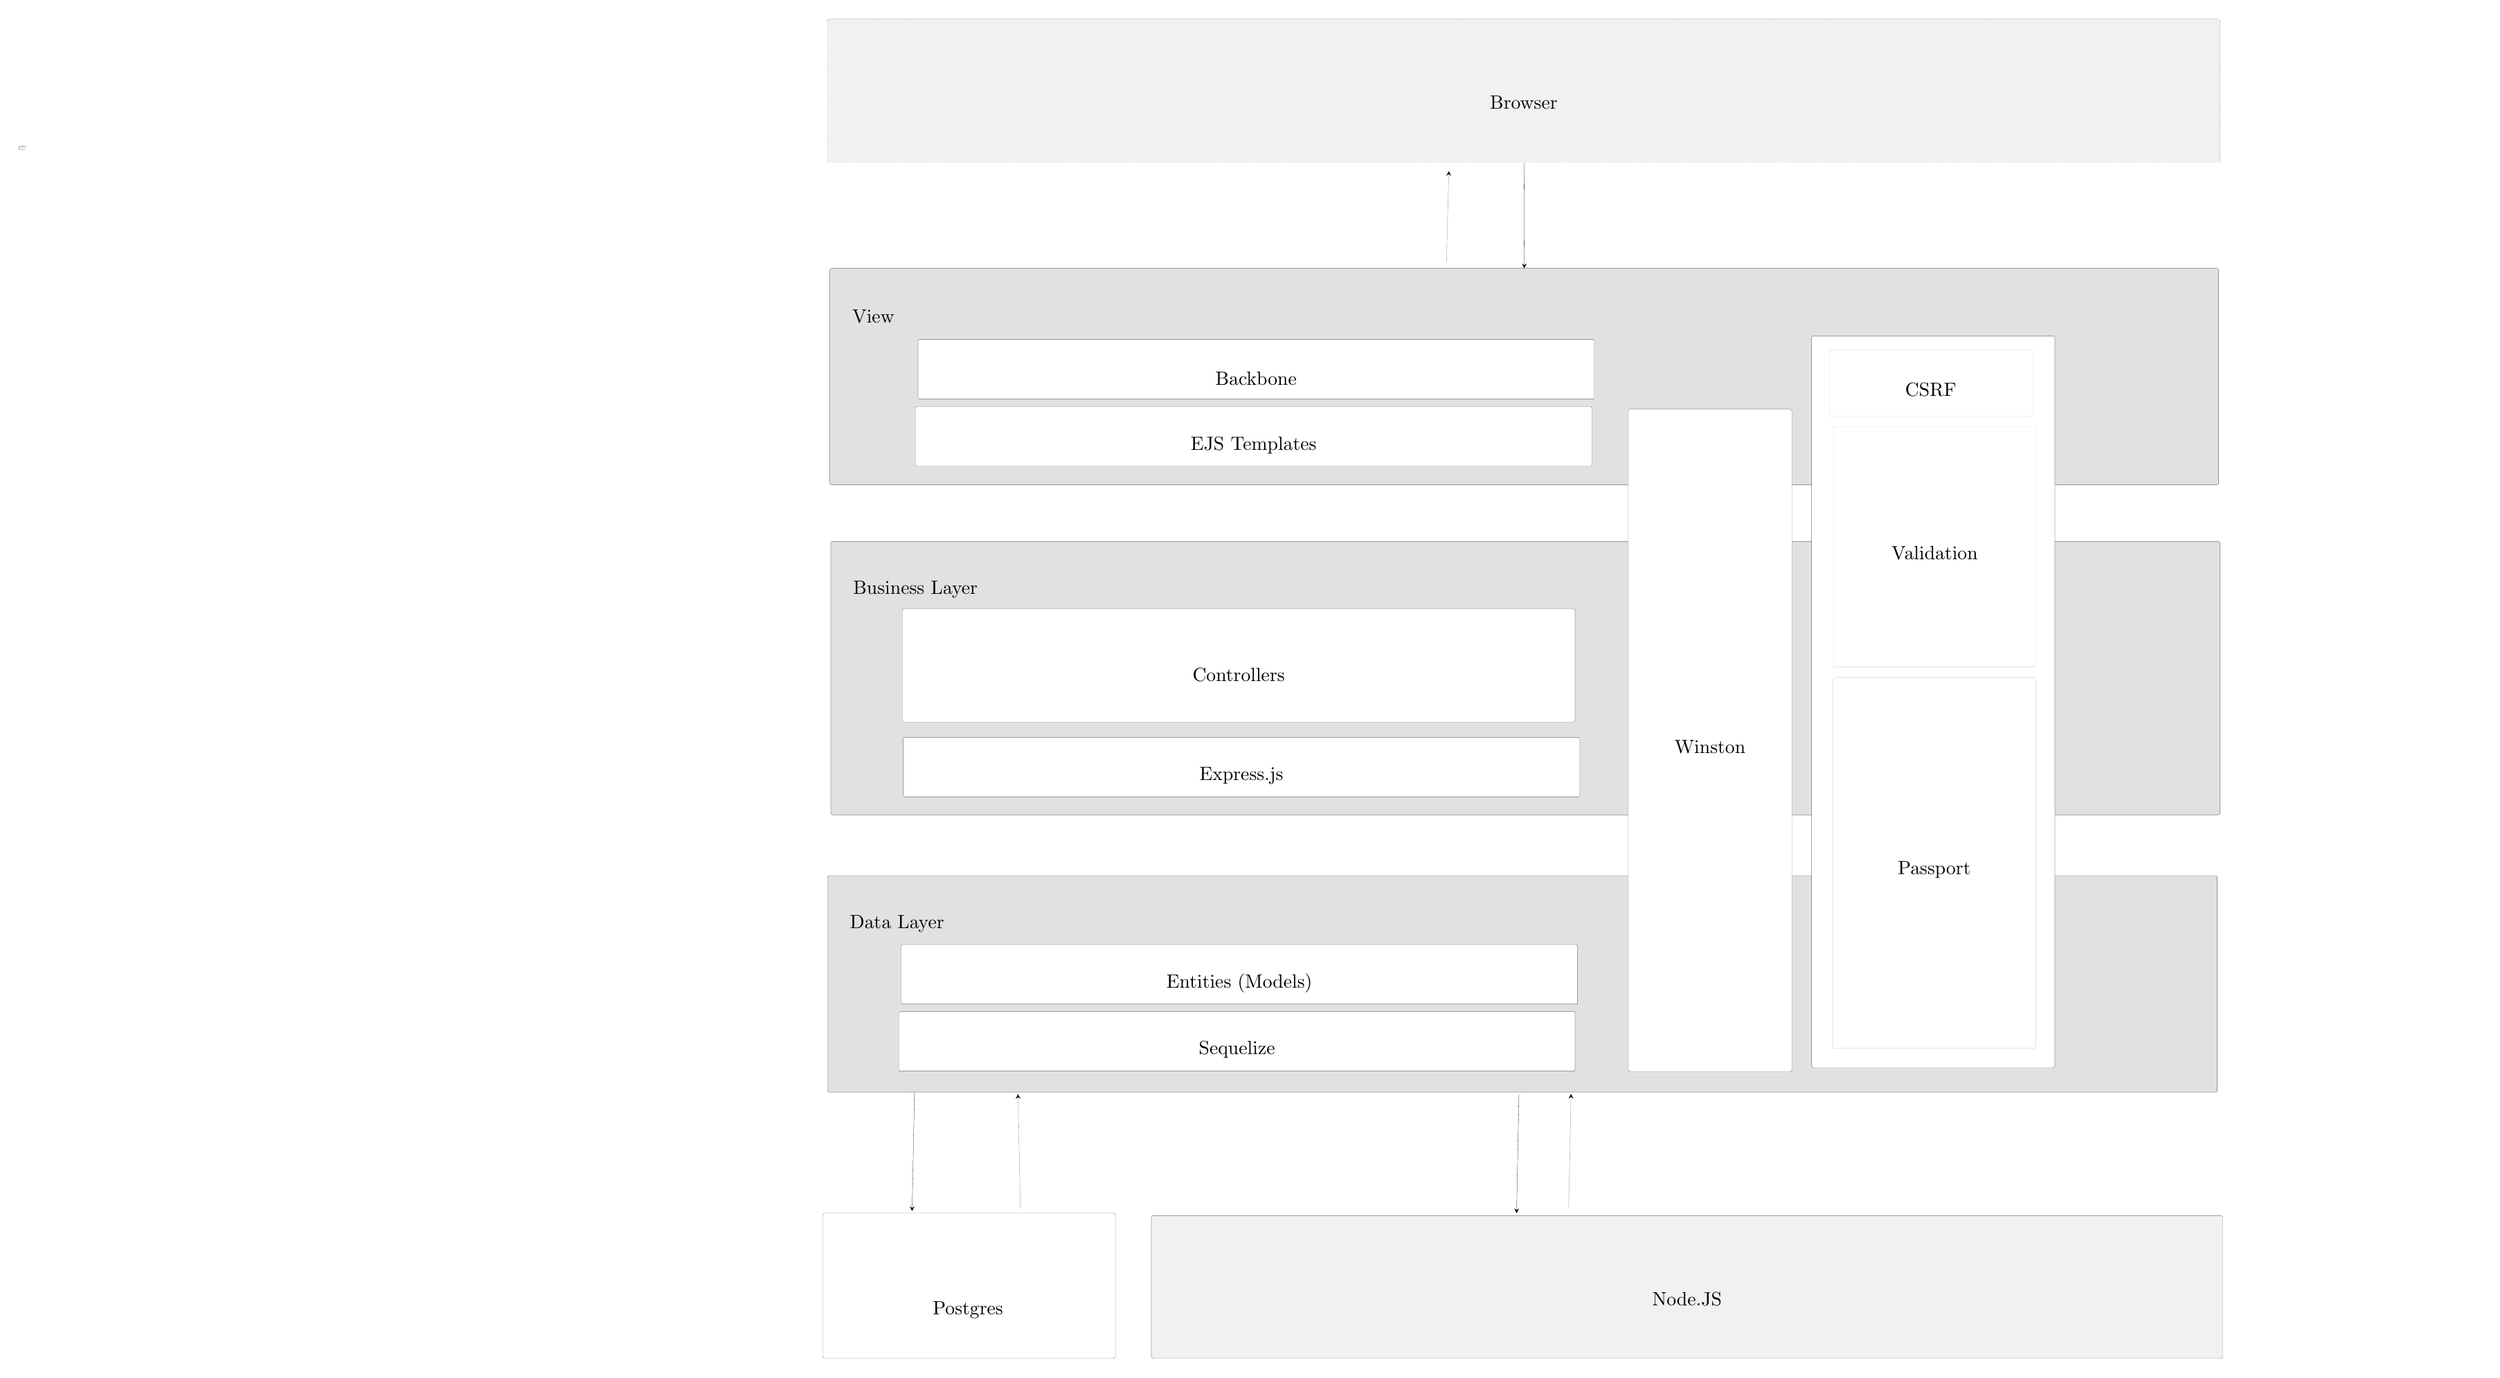
\begin{tikzpicture}
\pgftransformxscale{1.000000}
\pgftransformyscale{-1.000000}
\definecolor{dialinecolor}{rgb}{0.000000, 0.000000, 0.000000}
\pgfsetstrokecolor{dialinecolor}
\definecolor{dialinecolor}{rgb}{1.000000, 1.000000, 1.000000}
\pgfsetfillcolor{dialinecolor}
% setfont left to latex
\definecolor{dialinecolor}{rgb}{0.000000, 0.000000, 0.000000}
\pgfsetstrokecolor{dialinecolor}
\node[anchor=west] at (45.479400\du,9.979680\du){};
\pgfsetlinewidth{0.050000\du}
\pgfsetdash{}{0pt}
\pgfsetdash{}{0pt}
\pgfsetroundjoin
{\pgfsetcornersarced{\pgfpoint{1.000000\du}{1.000000\du}}\definecolor{dialinecolor}{rgb}{0.882353, 0.882353, 0.882353}
\pgfsetfillcolor{dialinecolor}
\fill (15.448400\du,2.971250\du)--(15.448400\du,6.945606\du)--(40.925000\du,6.945606\du)--(40.925000\du,2.971250\du)--cycle;
}{\pgfsetcornersarced{\pgfpoint{1.000000\du}{1.000000\du}}\definecolor{dialinecolor}{rgb}{0.000000, 0.000000, 0.000000}
\pgfsetstrokecolor{dialinecolor}
\draw (15.448400\du,2.971250\du)--(15.448400\du,6.945606\du)--(40.925000\du,6.945606\du)--(40.925000\du,2.971250\du)--cycle;
}\pgfsetlinewidth{0.050000\du}
\pgfsetdash{}{0pt}
\pgfsetdash{}{0pt}
\pgfsetroundjoin
{\pgfsetcornersarced{\pgfpoint{1.000000\du}{1.000000\du}}\definecolor{dialinecolor}{rgb}{0.882353, 0.882353, 0.882353}
\pgfsetfillcolor{dialinecolor}
\fill (15.403600\du,14.115700\du)--(15.403600\du,18.090056\du)--(40.900000\du,18.090056\du)--(40.900000\du,14.115700\du)--cycle;
}{\pgfsetcornersarced{\pgfpoint{1.000000\du}{1.000000\du}}\definecolor{dialinecolor}{rgb}{0.000000, 0.000000, 0.000000}
\pgfsetstrokecolor{dialinecolor}
\draw (15.403600\du,14.115700\du)--(15.403600\du,18.090056\du)--(40.900000\du,18.090056\du)--(40.900000\du,14.115700\du)--cycle;
}\pgfsetlinewidth{0.050000\du}
\pgfsetdash{}{0pt}
\pgfsetdash{}{0pt}
\pgfsetroundjoin
{\pgfsetcornersarced{\pgfpoint{1.000000\du}{1.000000\du}}\definecolor{dialinecolor}{rgb}{0.882353, 0.882353, 0.882353}
\pgfsetfillcolor{dialinecolor}
\fill (15.464700\du,7.983850\du)--(15.464700\du,13.000002\du)--(40.950000\du,13.000002\du)--(40.950000\du,7.983850\du)--cycle;
}{\pgfsetcornersarced{\pgfpoint{1.000000\du}{1.000000\du}}\definecolor{dialinecolor}{rgb}{0.000000, 0.000000, 0.000000}
\pgfsetstrokecolor{dialinecolor}
\draw (15.464700\du,7.983850\du)--(15.464700\du,13.000002\du)--(40.950000\du,13.000002\du)--(40.950000\du,7.983850\du)--cycle;
}% setfont left to latex
\definecolor{dialinecolor}{rgb}{0.000000, 0.000000, 0.000000}
\pgfsetstrokecolor{dialinecolor}
\node[anchor=west] at (15.741293\du,3.859143\du){View};
% setfont left to latex
\definecolor{dialinecolor}{rgb}{0.000000, 0.000000, 0.000000}
\pgfsetstrokecolor{dialinecolor}
\node[anchor=west] at (15.757593\du,8.871743\du){Business Layer};
% setfont left to latex
\definecolor{dialinecolor}{rgb}{0.000000, 0.000000, 0.000000}
\pgfsetstrokecolor{dialinecolor}
\node[anchor=west] at (15.696493\du,15.003593\du){Data Layer};
\pgfsetlinewidth{0.050000\du}
\pgfsetdash{}{0pt}
\pgfsetdash{}{0pt}
\pgfsetroundjoin
{\pgfsetcornersarced{\pgfpoint{1.000000\du}{1.000000\du}}\definecolor{dialinecolor}{rgb}{0.945098, 0.945098, 0.945098}
\pgfsetfillcolor{dialinecolor}
\fill (21.344500\du,20.353600\du)--(21.344500\du,22.974055\du)--(41.000030\du,22.974055\du)--(41.000030\du,20.353600\du)--cycle;
}{\pgfsetcornersarced{\pgfpoint{1.000000\du}{1.000000\du}}\definecolor{dialinecolor}{rgb}{0.000000, 0.000000, 0.000000}
\pgfsetstrokecolor{dialinecolor}
\draw (21.344500\du,20.353600\du)--(21.344500\du,22.974055\du)--(41.000030\du,22.974055\du)--(41.000030\du,20.353600\du)--cycle;
}% setfont left to latex
\definecolor{dialinecolor}{rgb}{0.000000, 0.000000, 0.000000}
\pgfsetstrokecolor{dialinecolor}
\node at (31.172200\du,21.886300\du){Node.JS};
\pgfsetlinewidth{0.050000\du}
\pgfsetdash{}{0pt}
\pgfsetdash{}{0pt}
\pgfsetroundjoin
{\pgfsetcornersarced{\pgfpoint{0.500000\du}{0.500000\du}}\definecolor{dialinecolor}{rgb}{1.000000, 1.000000, 1.000000}
\pgfsetfillcolor{dialinecolor}
\fill (17.064400\du,4.281480\du)--(17.064400\du,5.373336\du)--(29.467885\du,5.373336\du)--(29.467885\du,4.281480\du)--cycle;
}{\pgfsetcornersarced{\pgfpoint{0.500000\du}{0.500000\du}}\definecolor{dialinecolor}{rgb}{0.000000, 0.000000, 0.000000}
\pgfsetstrokecolor{dialinecolor}
\draw (17.064400\du,4.281480\du)--(17.064400\du,5.373336\du)--(29.467885\du,5.373336\du)--(29.467885\du,4.281480\du)--cycle;
}\pgfsetlinewidth{0.050000\du}
\pgfsetdash{}{0pt}
\pgfsetdash{}{0pt}
\pgfsetroundjoin
{\pgfsetcornersarced{\pgfpoint{0.500000\du}{0.500000\du}}\definecolor{dialinecolor}{rgb}{1.000000, 1.000000, 1.000000}
\pgfsetfillcolor{dialinecolor}
\fill (17.019500\du,5.511890\du)--(17.019500\du,6.603746\du)--(29.422985\du,6.603746\du)--(29.422985\du,5.511890\du)--cycle;
}{\pgfsetcornersarced{\pgfpoint{0.500000\du}{0.500000\du}}\definecolor{dialinecolor}{rgb}{0.000000, 0.000000, 0.000000}
\pgfsetstrokecolor{dialinecolor}
\draw (17.019500\du,5.511890\du)--(17.019500\du,6.603746\du)--(29.422985\du,6.603746\du)--(29.422985\du,5.511890\du)--cycle;
}% setfont left to latex
\definecolor{dialinecolor}{rgb}{0.000000, 0.000000, 0.000000}
\pgfsetstrokecolor{dialinecolor}
\node at (23.266100\du,4.991160\du){Backbone};
% setfont left to latex
\definecolor{dialinecolor}{rgb}{0.000000, 0.000000, 0.000000}
\pgfsetstrokecolor{dialinecolor}
\node[anchor=west] at (23.221300\du,6.057810\du){};
% setfont left to latex
\definecolor{dialinecolor}{rgb}{0.000000, 0.000000, 0.000000}
\pgfsetstrokecolor{dialinecolor}
\node at (23.221300\du,6.221560\du){EJS Templates};
\pgfsetlinewidth{0.050000\du}
\pgfsetdash{}{0pt}
\pgfsetdash{}{0pt}
\pgfsetroundjoin
{\pgfsetcornersarced{\pgfpoint{0.500000\du}{0.500000\du}}\definecolor{dialinecolor}{rgb}{1.000000, 1.000000, 1.000000}
\pgfsetfillcolor{dialinecolor}
\fill (16.777324\du,9.224200\du)--(16.777324\du,11.296437\du)--(29.117315\du,11.296437\du)--(29.117315\du,9.224200\du)--cycle;
}{\pgfsetcornersarced{\pgfpoint{0.500000\du}{0.500000\du}}\definecolor{dialinecolor}{rgb}{0.000000, 0.000000, 0.000000}
\pgfsetstrokecolor{dialinecolor}
\draw (16.777324\du,9.224200\du)--(16.777324\du,11.296437\du)--(29.117315\du,11.296437\du)--(29.117315\du,9.224200\du)--cycle;
}% setfont left to latex
\definecolor{dialinecolor}{rgb}{0.000000, 0.000000, 0.000000}
\pgfsetstrokecolor{dialinecolor}
\node at (22.947320\du,10.424069\du){Controllers};
\pgfsetlinewidth{0.050000\du}
\pgfsetdash{}{0pt}
\pgfsetdash{}{0pt}
\pgfsetroundjoin
{\pgfsetcornersarced{\pgfpoint{1.000000\du}{1.000000\du}}\definecolor{dialinecolor}{rgb}{1.000000, 1.000000, 1.000000}
\pgfsetfillcolor{dialinecolor}
\fill (30.093829\du,5.555635\du)--(30.093829\du,17.710427\du)--(33.093829\du,17.710427\du)--(33.093829\du,5.555635\du)--cycle;
}{\pgfsetcornersarced{\pgfpoint{1.000000\du}{1.000000\du}}\definecolor{dialinecolor}{rgb}{0.000000, 0.000000, 0.000000}
\pgfsetstrokecolor{dialinecolor}
\draw (30.093829\du,5.555635\du)--(30.093829\du,17.710427\du)--(33.093829\du,17.710427\du)--(33.093829\du,5.555635\du)--cycle;
}% setfont left to latex
\definecolor{dialinecolor}{rgb}{0.000000, 0.000000, 0.000000}
\pgfsetstrokecolor{dialinecolor}
\node at (31.593829\du,11.756781\du){Winston};
\pgfsetlinewidth{0.050000\du}
\pgfsetdash{}{0pt}
\pgfsetdash{}{0pt}
\pgfsetroundjoin
{\pgfsetcornersarced{\pgfpoint{0.500000\du}{0.500000\du}}\definecolor{dialinecolor}{rgb}{1.000000, 1.000000, 1.000000}
\pgfsetfillcolor{dialinecolor}
\fill (16.758700\du,15.382300\du)--(16.758700\du,16.474156\du)--(29.162185\du,16.474156\du)--(29.162185\du,15.382300\du)--cycle;
}{\pgfsetcornersarced{\pgfpoint{0.500000\du}{0.500000\du}}\definecolor{dialinecolor}{rgb}{0.000000, 0.000000, 0.000000}
\pgfsetstrokecolor{dialinecolor}
\draw (16.758700\du,15.382300\du)--(16.758700\du,16.474156\du)--(29.162185\du,16.474156\du)--(29.162185\du,15.382300\du)--cycle;
}\pgfsetlinewidth{0.050000\du}
\pgfsetdash{}{0pt}
\pgfsetdash{}{0pt}
\pgfsetroundjoin
{\pgfsetcornersarced{\pgfpoint{0.500000\du}{0.500000\du}}\definecolor{dialinecolor}{rgb}{1.000000, 1.000000, 1.000000}
\pgfsetfillcolor{dialinecolor}
\fill (16.713800\du,16.612700\du)--(16.713800\du,17.704556\du)--(29.117285\du,17.704556\du)--(29.117285\du,16.612700\du)--cycle;
}{\pgfsetcornersarced{\pgfpoint{0.500000\du}{0.500000\du}}\definecolor{dialinecolor}{rgb}{0.000000, 0.000000, 0.000000}
\pgfsetstrokecolor{dialinecolor}
\draw (16.713800\du,16.612700\du)--(16.713800\du,17.704556\du)--(29.117285\du,17.704556\du)--(29.117285\du,16.612700\du)--cycle;
}% setfont left to latex
\definecolor{dialinecolor}{rgb}{0.000000, 0.000000, 0.000000}
\pgfsetstrokecolor{dialinecolor}
\node at (22.960400\du,16.091950\du){Entities (Models)};
% setfont left to latex
\definecolor{dialinecolor}{rgb}{0.000000, 0.000000, 0.000000}
\pgfsetstrokecolor{dialinecolor}
\node at (22.915500\du,17.315506\du){Sequelize};
\pgfsetlinewidth{0.050000\du}
\pgfsetdash{}{0pt}
\pgfsetdash{}{0pt}
\pgfsetroundjoin
{\pgfsetcornersarced{\pgfpoint{1.000000\du}{1.000000\du}}\definecolor{dialinecolor}{rgb}{1.000000, 1.000000, 1.000000}
\pgfsetfillcolor{dialinecolor}
\fill (15.317400\du,20.309900\du)--(15.317400\du,22.974029\du)--(20.689332\du,22.974029\du)--(20.689332\du,20.309900\du)--cycle;
}{\pgfsetcornersarced{\pgfpoint{1.000000\du}{1.000000\du}}\definecolor{dialinecolor}{rgb}{0.000000, 0.000000, 0.000000}
\pgfsetstrokecolor{dialinecolor}
\draw (15.317400\du,20.309900\du)--(15.317400\du,22.974029\du)--(20.689332\du,22.974029\du)--(20.689332\du,20.309900\du)--cycle;
}\pgfsetlinewidth{0.050000\du}
\pgfsetdash{}{0pt}
\pgfsetdash{}{0pt}
\pgfsetbuttcap
\pgfsetmiterjoin
\pgfsetlinewidth{0.050000\du}
\pgfsetbuttcap
\pgfsetmiterjoin
\pgfsetdash{}{0pt}
\definecolor{dialinecolor}{rgb}{1.000000, 1.000000, 1.000000}
\pgfsetfillcolor{dialinecolor}
\pgfpathmoveto{\pgfpoint{16.427800\du}{20.969667\du}}
\pgfpathcurveto{\pgfpoint{17.049300\du}{20.694667\du}}{\pgfpoint{17.360050\du}{20.603000\du}}{\pgfpoint{17.981550\du}{20.603000\du}}
\pgfpathcurveto{\pgfpoint{18.603050\du}{20.603000\du}}{\pgfpoint{18.913800\du}{20.694667\du}}{\pgfpoint{19.535300\du}{20.969667\du}}
\pgfpathlineto{\pgfpoint{19.535300\du}{22.436333\du}}
\pgfpathcurveto{\pgfpoint{18.913800\du}{22.711333\du}}{\pgfpoint{18.603050\du}{22.803000\du}}{\pgfpoint{17.981550\du}{22.803000\du}}
\pgfpathcurveto{\pgfpoint{17.360050\du}{22.803000\du}}{\pgfpoint{17.049300\du}{22.711333\du}}{\pgfpoint{16.427800\du}{22.436333\du}}
\pgfpathlineto{\pgfpoint{16.427800\du}{20.969667\du}}
\pgfusepath{fill}
\definecolor{dialinecolor}{rgb}{0.000000, 0.000000, 0.000000}
\pgfsetstrokecolor{dialinecolor}
\pgfpathmoveto{\pgfpoint{16.427800\du}{20.969667\du}}
\pgfpathcurveto{\pgfpoint{17.049300\du}{20.694667\du}}{\pgfpoint{17.360050\du}{20.603000\du}}{\pgfpoint{17.981550\du}{20.603000\du}}
\pgfpathcurveto{\pgfpoint{18.603050\du}{20.603000\du}}{\pgfpoint{18.913800\du}{20.694667\du}}{\pgfpoint{19.535300\du}{20.969667\du}}
\pgfpathlineto{\pgfpoint{19.535300\du}{22.436333\du}}
\pgfpathcurveto{\pgfpoint{18.913800\du}{22.711333\du}}{\pgfpoint{18.603050\du}{22.803000\du}}{\pgfpoint{17.981550\du}{22.803000\du}}
\pgfpathcurveto{\pgfpoint{17.360050\du}{22.803000\du}}{\pgfpoint{17.049300\du}{22.711333\du}}{\pgfpoint{16.427800\du}{22.436333\du}}
\pgfpathlineto{\pgfpoint{16.427800\du}{20.969667\du}}
\pgfusepath{stroke}
\pgfsetbuttcap
\pgfsetmiterjoin
\pgfsetdash{}{0pt}
\definecolor{dialinecolor}{rgb}{0.000000, 0.000000, 0.000000}
\pgfsetstrokecolor{dialinecolor}
\pgfpathmoveto{\pgfpoint{16.427800\du}{20.969667\du}}
\pgfpathcurveto{\pgfpoint{17.049300\du}{21.244667\du}}{\pgfpoint{17.360050\du}{21.336333\du}}{\pgfpoint{17.981550\du}{21.336333\du}}
\pgfpathcurveto{\pgfpoint{18.603050\du}{21.336333\du}}{\pgfpoint{18.913800\du}{21.244667\du}}{\pgfpoint{19.535300\du}{20.969667\du}}
\pgfusepath{stroke}
% setfont left to latex
\definecolor{dialinecolor}{rgb}{0.000000, 0.000000, 0.000000}
\pgfsetstrokecolor{dialinecolor}
\node at (17.981550\du,22.086333\du){Postgres};
\pgfsetlinewidth{0.100000\du}
\pgfsetdash{}{0pt}
\pgfsetdash{}{0pt}
\pgfsetbuttcap
{
\definecolor{dialinecolor}{rgb}{0.000000, 0.000000, 0.000000}
\pgfsetfillcolor{dialinecolor}
% was here!!!
\pgfsetarrowsend{stealth}
\definecolor{dialinecolor}{rgb}{0.000000, 0.000000, 0.000000}
\pgfsetstrokecolor{dialinecolor}
\draw (28.088100\du,18.126200\du)--(28.044400\du,20.309900\du);
}
\pgfsetlinewidth{0.100000\du}
\pgfsetdash{{\pgflinewidth}{0.200000\du}}{0cm}
\pgfsetdash{{\pgflinewidth}{0.200000\du}}{0cm}
\pgfsetbuttcap
{
\definecolor{dialinecolor}{rgb}{0.000000, 0.000000, 0.000000}
\pgfsetfillcolor{dialinecolor}
% was here!!!
\pgfsetarrowsend{stealth}
\definecolor{dialinecolor}{rgb}{0.000000, 0.000000, 0.000000}
\pgfsetstrokecolor{dialinecolor}
\draw (29.000000\du,20.218400\du)--(29.043700\du,18.122000\du);
}
\pgfsetlinewidth{0.100000\du}
\pgfsetdash{{\pgflinewidth}{0.200000\du}}{0cm}
\pgfsetdash{{\pgflinewidth}{0.200000\du}}{0cm}
\pgfsetbuttcap
{
\definecolor{dialinecolor}{rgb}{0.000000, 0.000000, 0.000000}
\pgfsetfillcolor{dialinecolor}
% was here!!!
\pgfsetarrowsend{stealth}
\definecolor{dialinecolor}{rgb}{0.000000, 0.000000, 0.000000}
\pgfsetstrokecolor{dialinecolor}
\draw (18.942400\du,20.222600\du)--(18.898700\du,18.126200\du);
}
\pgfsetlinewidth{0.050000\du}
\pgfsetdash{}{0pt}
\pgfsetdash{}{0pt}
\pgfsetroundjoin
{\pgfsetcornersarced{\pgfpoint{1.000000\du}{1.000000\du}}\definecolor{dialinecolor}{rgb}{1.000000, 1.000000, 1.000000}
\pgfsetfillcolor{dialinecolor}
\fill (33.457433\du,4.212132\du)--(33.457433\du,17.639717\du)--(37.918555\du,17.639717\du)--(37.918555\du,4.212132\du)--cycle;
}{\pgfsetcornersarced{\pgfpoint{1.000000\du}{1.000000\du}}\definecolor{dialinecolor}{rgb}{0.000000, 0.000000, 0.000000}
\pgfsetstrokecolor{dialinecolor}
\draw (33.457433\du,4.212132\du)--(33.457433\du,17.639717\du)--(37.918555\du,17.639717\du)--(37.918555\du,4.212132\du)--cycle;
}\pgfsetlinewidth{0.050000\du}
\pgfsetdash{{\pgflinewidth}{0.200000\du}}{0cm}
\pgfsetdash{{\pgflinewidth}{0.200000\du}}{0cm}
\pgfsetroundjoin
{\pgfsetcornersarced{\pgfpoint{1.000000\du}{1.000000\du}}\definecolor{dialinecolor}{rgb}{0.945098, 0.945098, 0.945098}
\pgfsetfillcolor{dialinecolor}
\fill (15.403600\du,-1.598430\du)--(15.403600\du,1.022025\du)--(40.950000\du,1.022025\du)--(40.950000\du,-1.598430\du)--cycle;
}{\pgfsetcornersarced{\pgfpoint{1.000000\du}{1.000000\du}}\definecolor{dialinecolor}{rgb}{0.000000, 0.000000, 0.000000}
\pgfsetstrokecolor{dialinecolor}
\draw (15.403600\du,-1.598430\du)--(15.403600\du,1.022025\du)--(40.950000\du,1.022025\du)--(40.950000\du,-1.598430\du)--cycle;
}% setfont left to latex
\definecolor{dialinecolor}{rgb}{0.000000, 0.000000, 0.000000}
\pgfsetstrokecolor{dialinecolor}
\node at (28.176800\du,-0.065703\du){Browser};
\pgfsetlinewidth{0.100000\du}
\pgfsetdash{}{0pt}
\pgfsetdash{}{0pt}
\pgfsetbuttcap
{
\definecolor{dialinecolor}{rgb}{0.000000, 0.000000, 0.000000}
\pgfsetfillcolor{dialinecolor}
% was here!!!
\pgfsetarrowsend{stealth}
\definecolor{dialinecolor}{rgb}{0.000000, 0.000000, 0.000000}
\pgfsetstrokecolor{dialinecolor}
\draw (28.180853\du,1.046295\du)--(28.186700\du,2.971250\du);
}
\pgfsetlinewidth{0.100000\du}
\pgfsetdash{{\pgflinewidth}{0.200000\du}}{0cm}
\pgfsetdash{{\pgflinewidth}{0.200000\du}}{0cm}
\pgfsetbuttcap
{
\definecolor{dialinecolor}{rgb}{0.000000, 0.000000, 0.000000}
\pgfsetfillcolor{dialinecolor}
% was here!!!
\pgfsetarrowsend{stealth}
\definecolor{dialinecolor}{rgb}{0.000000, 0.000000, 0.000000}
\pgfsetstrokecolor{dialinecolor}
\draw (26.758300\du,2.848810\du)--(26.802000\du,1.189190\du);
}
\pgfsetlinewidth{0.050000\du}
\pgfsetdash{}{0pt}
\pgfsetdash{}{0pt}
\pgfsetroundjoin
{\pgfsetcornersarced{\pgfpoint{0.800000\du}{0.800000\du}}\definecolor{dialinecolor}{rgb}{1.000000, 1.000000, 1.000000}
\pgfsetfillcolor{dialinecolor}
\fill (33.850533\du,10.479720\du)--(33.850533\du,17.286163\du)--(37.565002\du,17.286163\du)--(37.565002\du,10.479720\du)--cycle;
}{\pgfsetcornersarced{\pgfpoint{0.800000\du}{0.800000\du}}\definecolor{dialinecolor}{rgb}{0.674510, 0.666667, 0.666667}
\pgfsetstrokecolor{dialinecolor}
\draw (33.850533\du,10.479720\du)--(33.850533\du,17.286163\du)--(37.565002\du,17.286163\du)--(37.565002\du,10.479720\du)--cycle;
}% setfont left to latex
\definecolor{dialinecolor}{rgb}{0.000000, 0.000000, 0.000000}
\pgfsetstrokecolor{dialinecolor}
\node at (35.707768\du,14.006692\du){Passport};
\pgfsetlinewidth{0.050000\du}
\pgfsetdash{}{0pt}
\pgfsetdash{}{0pt}
\pgfsetroundjoin
{\pgfsetcornersarced{\pgfpoint{0.500000\du}{0.500000\du}}\definecolor{dialinecolor}{rgb}{1.000000, 1.000000, 1.000000}
\pgfsetfillcolor{dialinecolor}
\fill (16.794445\du,11.577813\du)--(16.794445\du,12.669669\du)--(29.197929\du,12.669669\du)--(29.197929\du,11.577813\du)--cycle;
}{\pgfsetcornersarced{\pgfpoint{0.500000\du}{0.500000\du}}\definecolor{dialinecolor}{rgb}{0.000000, 0.000000, 0.000000}
\pgfsetstrokecolor{dialinecolor}
\draw (16.794445\du,11.577813\du)--(16.794445\du,12.669669\du)--(29.197929\du,12.669669\du)--(29.197929\du,11.577813\du)--cycle;
}% setfont left to latex
\definecolor{dialinecolor}{rgb}{0.000000, 0.000000, 0.000000}
\pgfsetstrokecolor{dialinecolor}
\node at (22.996187\du,12.287491\du){Express.js};
\pgfsetlinewidth{0.100000\du}
\pgfsetdash{}{0pt}
\pgfsetdash{}{0pt}
\pgfsetbuttcap
{
\definecolor{dialinecolor}{rgb}{0.000000, 0.000000, 0.000000}
\pgfsetfillcolor{dialinecolor}
% was here!!!
\pgfsetarrowsend{stealth}
\definecolor{dialinecolor}{rgb}{0.000000, 0.000000, 0.000000}
\pgfsetstrokecolor{dialinecolor}
\draw (17.000000\du,18.087300\du)--(16.956300\du,20.271100\du);
}
\pgfsetlinewidth{0.050000\du}
\pgfsetdash{}{0pt}
\pgfsetdash{}{0pt}
\pgfsetroundjoin
{\pgfsetcornersarced{\pgfpoint{0.500000\du}{0.500000\du}}\definecolor{dialinecolor}{rgb}{1.000000, 1.000000, 1.000000}
\pgfsetfillcolor{dialinecolor}
\fill (33.785767\du,4.463033\du)--(33.785767\du,5.689612\du)--(37.500236\du,5.689612\du)--(37.500236\du,4.463033\du)--cycle;
}{\pgfsetcornersarced{\pgfpoint{0.500000\du}{0.500000\du}}\definecolor{dialinecolor}{rgb}{0.674510, 0.666667, 0.666667}
\pgfsetstrokecolor{dialinecolor}
\draw (33.785767\du,4.463033\du)--(33.785767\du,5.689612\du)--(37.500236\du,5.689612\du)--(37.500236\du,4.463033\du)--cycle;
}% setfont left to latex
\definecolor{dialinecolor}{rgb}{0.000000, 0.000000, 0.000000}
\pgfsetstrokecolor{dialinecolor}
\node at (35.643002\du,5.200073\du){CSRF};
\pgfsetlinewidth{0.050000\du}
\pgfsetdash{}{0pt}
\pgfsetdash{}{0pt}
\pgfsetroundjoin
{\pgfsetcornersarced{\pgfpoint{0.500000\du}{0.500000\du}}\definecolor{dialinecolor}{rgb}{1.000000, 1.000000, 1.000000}
\pgfsetfillcolor{dialinecolor}
\fill (33.856478\du,5.877247\du)--(33.856478\du,10.285806\du)--(37.570947\du,10.285806\du)--(37.570947\du,5.877247\du)--cycle;
}{\pgfsetcornersarced{\pgfpoint{0.500000\du}{0.500000\du}}\definecolor{dialinecolor}{rgb}{0.674510, 0.666667, 0.666667}
\pgfsetstrokecolor{dialinecolor}
\draw (33.856478\du,5.877247\du)--(33.856478\du,10.285806\du)--(37.570947\du,10.285806\du)--(37.570947\du,5.877247\du)--cycle;
}% setfont left to latex
\definecolor{dialinecolor}{rgb}{0.000000, 0.000000, 0.000000}
\pgfsetstrokecolor{dialinecolor}
\node at (35.713712\du,8.200058\du){Validation};
\end{tikzpicture}

	}

	\caption{Software Layers}
\end{figure}

\subsubsection*{Client-Side MVC}
Auf der Client-Seite im Browser wird ebenfalls das MVC-Pattern \cite{MVC} verwendet. Dies ermöglicht eine entkoppelte Implementation.\\
Das Client-Side MVC ist auf Backbone.js \cite{Backbonejs} aufgebaut.

\subsubsection*{Handlebars Views}
Die Präsentations-Schicht verwendet Handlebars \cite{Handlebars}. Dieses Templating-System forciert die Library-Benutzer zu quasi Logikfreien Templates.

\subsubsection*{Winston}
Winston \cite{Winston} ist ein Logging-Framework für \gls{nodejs}.

\subsubsection*{CSRF}
\gls{CSRF}-Schicht um CSRF-Attacken zu verhindern. Dies wird von Express zur Verfügung \cite{ExpressjsCSRF} gestellt und muss in der Applikation aktiviert werden.

\subsubsection*{Validation}
Formular-Inhalte werden durch ``node-validator'' \cite{nodevalidator} auf vorher definierte Bedingungen überprüft und gereinigt (sanitized).

\subsubsection*{Passport}
Passport \cite{Passportjs} ist ein authentication-Framework für \gls{nodejs}. Und ermöglicht durch verschiedene Strategien (Strategy-Pattern \cite{StrategyPattern}) das einloggen mittels z.B. Facebook-Connect \cite{FacebookConnect}.

\subsubsection*{Escaping}
Jede Datenbank-Query muss Escaped werden, damit keine invaliden User-Input Daten die Datenbank erreichen können. Das ORM Sequelize \cite{Sequelize} stellt dies zur Verfügung.